\documentclass[x11names]{article}
\usepackage{verbatim}
\usepackage{listings}
\usepackage{graphicx}
\usepackage{a4wide}
\usepackage{color}
\usepackage{amsmath}
\usepackage{amssymb}
\usepackage[dvips]{epsfig}
\usepackage[T1]{fontenc}
\usepackage{cite} % [2,3,4] --> [2--4]
\usepackage{shadow}
\usepackage{hyperref}
\usepackage{physics}
\usepackage{url}
\usepackage{tikz}
\usepackage{subcaption}
\usepackage[utf8]{inputenc}
\usepackage{booktabs} % Allows the use of \toprule, \midrule and \bottomrule in tables



%Tikz settings
\usetikzlibrary{shapes,arrows,chains}
% =================================================
% Set up a few colours
\colorlet{lcfree}{Green3}
\colorlet{lcnorm}{Blue3}
\colorlet{lccong}{Red3}
% -------------------------------------------------
% Set up a new layer for the debugging marks, and make sure it is on
% top
\pgfdeclarelayer{marx}
\pgfsetlayers{main,marx}
% A macro for marking coordinates (specific to the coordinate naming
% scheme used here). Swap the following 2 definitions to deactivate
% marks.
\providecommand{\cmark}[2][]{%
  \begin{pgfonlayer}{marx}
    \node [nmark] at (c#2#1) {#2};
  \end{pgfonlayer}{marx}
  } 
\providecommand{\cmark}[2][]{\relax} 



\setcounter{tocdepth}{2}

\lstset{language=c++}
\lstset{alsolanguage=[90]Fortran}
\lstset{basicstyle=\small}
\lstset{backgroundcolor=\color{white}}
\lstset{frame=single}
\lstset{stringstyle=\ttfamily}
\lstset{keywordstyle=\color{red}\bfseries}
\lstset{commentstyle=\itshape\color{blue}}
\lstset{showspaces=false}
\lstset{showstringspaces=false}
\lstset{showtabs=false}
\lstset{breaklines}


\title{ FYS-4411: Computational Physics II \\ Project 3 }
\author{Gullik Vetvik Killie\\
		Håkon Sebastian Bakke Mørk\\
		Jose Emilio Ruiz Navarro
		}

\begin{document}



\maketitle

\abstract{In this work, a simple Variational Monte Carlo (VMC) method has been used to calculate the values of the energies of the ground states of two atoms: Beryllium and Neon. The program uses importance sampling to improve efficiency and make the results more precise. To further improve the efficiency, MPI has been implemented as well. We provide a statistical analysis by the means of blocking so as to not understimate the error of our results. The one-body and charge densities were obtained to compare the effects of the Jastrow factor and provide insight into the electronic structure of the atoms.}

\tableofcontents

\section{Introduction}
VMC methods pose a very attractive alternative to other more complex ways of finding the ground state energies of simple atoms and molecules, like configuration-interaction calculations. The price to be paid in exchange for this simplicity is the sensitivity to the trial wave functions that are used, a VMC algorithm is very sensitive to how these are constructed, so they are one of the most important aspects to be considered (in this work, given the simple nature of the atoms which we will be working with, it's not so important to worry about the quality of the trial wave functions because very simple and basic ones are more than enough to reproduce the actual results). It shouldn't be forgotten that it is a variational method, and this implies that finding the optimal set of variational parameters is going to be the most important part of the calculation itself because it would create a lot of problems if the search range for the parameters was illy defined and not close enough to the variational minimum, namely, the results would have a poor quality in this case. This means that the parameters need to be chosen very carefully, or a recursive search with decreasingly coarse spacing in the space of variational parameters is required if there is no deep knowledge about the system in question.

Instead of evaluating a very complex multidimensional integral to compute the expectation value of an operator, like the hamiltonian in this case, a VMC calculation exploits the fact that the majority of the configuration space where the wave function belongs can be regarded as much less important than other parts, the values of the wave function are too small there and can be mostly ignored during the integration of the algorithm. To capitalize this, the Metropolis algorithm is added to the VMC method, as well as importance sampling.


\section{Theory}
	\subsection{Monte Carlo method with simple Metropolis sampling}
		In a quantum mechanical system the energy is given by the expectation value of the Hamiltonian, let \(\Psi_T\) be a proposal for a wavefunction that can describe the system.

		\begin{align}
			E[\hat{H}] = \expval{\hat{H}}{\Psi_T} = \frac{\int{d\vb{R} \Psi_T^*(\vb{R})\hat{H} \Psi_T(\vb{R})  }}{ \int{d\vb{R} \Psi_T^*(\vb{R}) \Psi_T(\vb{R}) }}
		\end{align}

		Let us introduce a local energy:

		\begin{align}
			E_L(\hat{H}) &= \frac{1}{ \Psi_T(\vb{R}) } \hat{H} \Psi_T(\vb{R}))
		\end{align}

		\begin{align}
			E[\hat{H}] &= \frac{\int{d\vb{R} \Psi_T^*(\vb{R}) \Psi_T(\vb{R}) E_L(\vb{R}))  }}{ \int{d\vb{R} \Psi_T^*(\vb{R}) \Psi_T(\vb{R}) }}
			\intertext{Since the denumerator is a scalar constant after integrating it we can put it inside the integral in the numerator}
			E[\hat{H}] &= \int{d\vb{R} \frac{\Psi_T^*(\vb{R}) \Psi_T(\vb{R})  }{\int{d\vb{R'} \Psi_T^*(\vb{R'}) \Psi_T(\vb{R'})}}  E_L(\vb{R})  }
			\\
			E[\hat{H}] &= \int{d\vb{R} P(\vb{R}) E_L(\vb{R}) }
		\end{align}

		This probability function with \(P(\vb{R})\) as the pdf, and we can use monte carlo integration to solve the integral.

		\begin{enumerate}
			\item Initialise system. Give particles a random position and decide how many Monte Carlo Cycles to run.
			\item Start Monte Carlo Calculations
				\begin{enumerate}
					\item Propose a move of the particles according to an algorithm, for example \newline \( \vb{R_{new}} = \vb{R_{old}} + \delta * r \), where \(r\) is a random number in \([0,1]\)
					\item Accept or reject move according to \( P(\vb{R_{new}})/ P(\vb{R_{old}}) \ge r \), where r is a new number. Update position values if accepted.
					\item Calculate energy for this cycle.
				\end{enumerate}
		\end{enumerate}

	\subsection{Helium atom}

		The dimensionless hamiltonian for the Helium atom consists of a kinetic energy part and a potential energy part and is given by

		\begin{align}
			\hat{H} &= -\frac{\nabla^2_1}{2} - \frac{\nabla^2_2}{2} - \frac{Z}{r_1} - \frac{Z}{r_2} + \frac{1}{r_{12}}
		\end{align}

		For the energy to be finite the wavefunction must be constructed so the local energy is finite at all points.

		\begin{align}
			E_L(r_i,r_{12}) &= \frac{1}{\Psi_T} \hat{H} \Psi_T
		\end{align}

		If we consider the case where \(r_i \rightarrow 0\) then the \(- \frac{\nabla^2_i}{2} - \frac{Z}{r_i} \) terms of the hamiltonian could cause the energy to blow up, so we need to make sure that those terms stay finite in the limit.

		\begin{align}
			\lim_{r_i\rightarrow 0} {E_L(r_1,r_{12}) } &= \frac{1}{R_i(r_i)} \left( - \frac{1}{2}\pdv[2]{}{x_k} - \frac{Z}{r_i} \right) R_i(r_i) + G(r_i, r_{ij})
			\\
			\lim_{r_i\rightarrow 0} {E_L(r_1,r_{12}) } &= \frac{1}{R_i(r_i)} \left( - \frac{1}{2}\pdv[2]{}{r_k} - \frac{1}{r_i}\pdv{}{r_i}	 -	 \frac{Z}{r_i} \right) R_i(r_i) + G(r_i, r_{ij})
			\intertext{ Derivatives of the wavefunction does not diverge since the wavefunction is finite at all points. so the following terms dominate when the particles approach the center. }
			\lim_{r_i\rightarrow 0} {E_L(r_1,r_{12}) } &= \frac{1}{R_i(r_i)} \left( - \frac{1}{r_i}\pdv{}{r_i}	 -	 \frac{Z}{r_i} \right) R_i(r_i)
			\end{align}

		\begin{align}
			 \frac{1}{R_i(r_i)} \pdv{}{r_i} R_i(r_i)	=  -Z  \qquad{ \text{ With solution }}  \qquad R_i(r_i) = A e^{-Z}
		\end{align}

		A similar calculation applies for \(r_{12} \rightarrow 0\) and a trialfunction of the form   \[\Psi_T(r_1,r_2,r_{12}) = e^{-\alpha (r_1 + r_2)} e^{\beta r_{12}} \] should fulfill the condition that the wavefunction is finite everywhere.

	\subsection{Beryllium atom}

		It is fairly simple to extend the calculational machinery of Variational
		Monte Carlo to other systems than the Helium atom. To show this we
		want to perform calculations on the beryllium atom. As beryllium has
		four electrons compared to the 2 of helium, we need to calculate a
		Slater determinant. However the computation of the Slater determinant
		can be simplified for beryllium. Sticking to hydrogen-like wave functions,
		we can write the trial wave function for beryllium as
		\begin{equation}
			\psi_{T}({\bf r_{1}},{\bf r_{2}},{\bf r_{3}},{\bf r_{4}})=Det\left(\phi_{1}({\bf r_{1}}),\phi_{2}({\bf r_{2}}),\phi_{3}({\bf r_{3}}),\phi_{4}({\bf r_{4}})\right)\prod_{i<j}^{4}\exp{\left(\frac{r_{ij}}{2(1+\beta r_{ij})}\right)},
			\label{eq:BerylliumTrialFunction}
		\end{equation}
		where $Det$ is a Slater determinant and the single-particle wave
		functions are the hydrogen wave functions for the 1s and 2s orbitals.
		With the variational ansatz these are
		\begin{align}
			\phi_{1s}({\bf r_{i}})=e^{-\alpha r_{i}},
		\end{align}
		and
		\begin{align}
			\phi_{2s}({\bf r_{i}})=\left(1-\alpha r_{i}/2\right)e^{-\alpha r_{i}/2}.
		\end{align}
		The Slater determinant is calculated using these ansatzes.

		Furthermore, for the Jastrow factor,
		\begin{align}
			\Psi_{C}=\prod_{i<j}g(r_{ij})=\exp{\sum_{i<j}\frac{ar_{ij}}{1+\beta r_{ij}}},
		\end{align}
		we need to take into account the spins of the electrons. We fix electrons
		1 and 2 to have spin up, and electron 3 and 4 to have spin down. This
		means that when the electrons have equal spins we get a factor
		\begin{align}
			a=\frac{1}{4},
		\end{align}
		and if they have opposite spins we get a factor
		\begin{align}
			a=\frac{1}{2}.
		\end{align}

	\subsection{Neon atom}

		Wishing to extend our variational Monte Carlo machinery further we implement Neon. Neon has ten electrons, so it is a big jump from Helium and Beryllium. Therefore we also have to implement a better way to handle the Slater determinant than we did in the previous project. The trial wave function for Neon can be written as
		\begin{equation}
		   \psi_{T}({\bf r_1},{\bf r_2}, \dots,{\bf r_{10}}) =
		   Det\left(\phi_{1}({\bf r_1}),\phi_{2}({\bf r_2}),
		   \dots,\phi_{10}({\bf r_{10}})\right)
		   \prod_{i<j}^{10}\exp{\left(\frac{r_{ij}}{2(1+\beta r_{ij})}\right)},
		   \label{eq:NeonTrialFunction}
		\end{equation}
		Now we need to include the $2p$ wave function as well. It is given as
		\begin{equation}
			\phi_{2p}({\bf r_i}) = \alpha {\bf r_i}e^{-\alpha r_i/2}.
		\end{equation}
		where $ {\bf r_i} = \sqrt{r_{i_x}^2+r_{i_y}^2+r_{i_z}^2}$.

	\subsection{Derivation of local energies}
		The local energy of is dependant on the Hamiltonian and the wavefunction describing the system, the Hamiltonian incorporates both a kinetic energy part given by \( \frac{\nabla_i^2}{2} \) for each particle
		and a potential energy part given by \(\frac{Z}{r_i}\) and \(\frac{1}{r_{ij}}\), where \(Z\) is the charge of the center, \(r_i\) is the distance for electron \(i\) to the atom center and \(r_{ij}\) is the distance between electron \(l\) and \(m\). Then the local energy is given by the following:

		\begin{align}
			E_L &= \sum_{i,i<j}{\frac{1}{ \Psi_T(\vb{r_i} , \vb{r_{ij}}) } \hat{H} \Psi_T(\vb{r_i} , \vb{r_{ij}})}
			\\
			&=	\sum_{i,i<j}\frac{1}{ \Psi_T(\vb{r_i} , \vb{r_{ij}}) } \left( - \frac{\nabla_i^2}{2} -\frac{Z}{r_i}  -  \frac{Z}{r_j} +  \frac{1}{r_{ij} }  \right) \Psi_T(\vb{r_i} , \vb{r_{ij}})
			\\
			&= \sum_{i,i<j}{-\frac{1}{2\Psi_T} \left(\nabla_i^2 \Psi_T  \right)  -\frac{Z}{r_i}  -  \frac{Z}{r_j} +  \frac{1}{r_{ij} }}
		\end{align}

		Let us change derivation variables:

		\begin{align}
			-\frac{1}{2\Psi_T} \left(\nabla_i^2 \Psi_T  \right) &= \sum_{m=1}^{3}{-\frac{1}{2\Psi_T} \left( \pdv[2]{\Psi_T}{x_m} \right)_i}
			\\
			&= \sum_{m=1}^{3}{-\frac{1}{2\Psi_T} \left( \pdv{}{x_m} \left( \pdv{\Psi_T}{r_i}\pdv{r_i}{x_m} \right) \right)_i}
			\intertext{Since \(r_i = \left( x_1^2 + x_2^2 + x_3^2 \right)^{1/2}\) then \( \pdv{r_i}{x_m} = \pdv{\left( x_1^2 + x_2^2 + x_3^2 \right)^{1/2}}{x_m} =\frac{x_m}{r_i} \)}
			&= \sum_{m=1}^{3}{-\frac{1}{2\Psi_T} \left( \pdv{}{x_m} \left( \pdv{\Psi_T}{r_i}\frac{x_m}{r_i} \right) \right)_i}
			\\
			&= \sum_{m=1}^{3}{-\frac{1}{2\Psi_T} \left( \pdv{\Psi_T}{x_m}{r_i}\frac{x_m}{r_i} + \pdv{\Psi_T}{r_i} \pdv{}{x_m} \left(\frac{x_m}{r_i} \right) \right)_i}
			\intertext{ The term \( \pdv{}{x_m} \left(\frac{x_m}{r_i} \right) \) becomes for the different values for \(m\),  \(\pdv{}{x_1}  \left( \frac{x_1}{\left( x_1^2 + x_2^2 + x_3^2 \right)^{1/2}} \right) = \frac{x_2^2 + x_3^2}{r_i^3}\) so all the values for \(m\) term it should sum up to \( \frac{ 2 (x_1^2 + x_2^2 + x_3^2) }{ r_i^3 } \) }
			&= -\frac{1}{2\Psi_T} \left( \pdv[2]{\Psi_T}{r_i}\frac{x_1^2 + x_2^2 + x_3^2}{r^2_i} + \pdv{\Psi_T}{r_i} \frac{ 2 (x_1^2 + x_2^2 + x_3^2) }{ r_i^3 } \right)_i
			\\
			&= -\frac{1}{2\Psi_T} \left( \pdv[2]{\Psi_T}{r_i} + \pdv{\Psi_T}{r_i} \frac{ 2 }{ r_i } \right)
		\end{align}
		Then the local energy becomes:
		\begin{align}
			E_L = \sum_{i,i<j}{  -\frac{1}{2\Psi_T} \left( \pdv[2]{\Psi_T}{r_i} + \pdv{\Psi_T}{r_i} \frac{ 2 }{ r_i } \right)  -\frac{Z}{r_i}  -  \frac{Z}{r_j} +  \frac{1}{r_{ij} }} \label{eq:localEnergy}
		\end{align}

		We can apply this to the simple helium trialfunction with no electronic interaction to obtain the local energy.

		\subsubsection{Helium: Simple trialfunction}
		The simple version of the trial function is only dependant on one parameter \( \alpha \) and does not take into account interaction between the two electrons, it is of the form
		\[ \Psi_T (\vb{r_1}, \vb{r_2}) = \exp{ -\alpha (r_1 + r_2) } \]Let us set this trialfunction into the equation for the local energy \eqref{eq:localEnergy}.
		\begin{align}
			E_L &= \sum_{i,i<j}{  -\frac{1}{2\Psi_T} \left( \pdv[2]{e^{-\alpha (r_i + r_j)}}{r_i} + \pdv{e^{-\alpha (r_i + r_j)}}{r_i} \frac{ 2 }{ r_i } \right)  -\frac{Z}{r_i}  -  \frac{Z}{r_j} +  \frac{1}{r_{ij} }}
			\\
			E_L &= -\frac{1}{2\Psi_T} \sum_{i=1}^2{ \left( \alpha^2 -\alpha \frac{ 2 }{ r_i } \right) \Psi_T  -\frac{Z}{r_i} +  \frac{1}{r_{ij} } }
			\\
			E_L &= -\alpha^2 + (\alpha-Z) \left( \frac{1}{r_1} + \frac{1}{r_2} \right) + \frac{1}{r_{12}}
		\end{align}

	\subsection{Calculating the Slater determinant}
		\subsubsection{Setting up the Slater determinant}
			To describe the wavefunction of multiple fermions we use a Slater
			determinant. The Slater determinant has the form
			\begin{align}
				\Phi(\mathbf{r}_{1},\mathbf{r}_{2},\mathbf{r}_{3},\mathbf{r}_{4},\alpha,\beta,\gamma,\delta)=\frac{1}{\sqrt{4!}}\left|\begin{array}{cccc}
				\psi_{100\uparrow}(\mathbf{r}_{1}) & \psi_{100\uparrow}(\mathbf{r}_{2}) & \psi_{100\uparrow}(\mathbf{r}_{3}) & \psi_{100\uparrow}(\mathbf{r}_{4})\\
				\psi_{100\downarrow}(\mathbf{r}_{1}) & \psi_{100\downarrow}(\mathbf{r}_{2}) & \psi_{100\downarrow}(\mathbf{r}_{3}) & \psi_{100\downarrow}(\mathbf{r}_{4})\\
				\psi_{200\uparrow}(\mathbf{r}_{1}) & \psi_{200\uparrow}(\mathbf{r}_{2}) & \psi_{200\uparrow}(\mathbf{r}_{3}) & \psi_{200\uparrow}(\mathbf{r}_{4})\\
				\psi_{200\downarrow}(\mathbf{r}_{1}) & \psi_{200\downarrow}(\mathbf{r}_{2}) & \psi_{200\downarrow}(\mathbf{r}_{3}) & \psi_{200\downarrow}(\mathbf{r}_{4})
				\end{array}\right|
			\end{align}
			for a four-fermionic system. Because the spatial wave functions for
			spin up and spin down states are equal, this Slater determinant equals
			zero. We can rewrite the Slater determinant as a product of two Slater
			determinants, one for spin up and one for spin down. This gives us
			\begin{eqnarray*}
				\Phi(\mathbf{r}_{1},\mathbf{r}_{2},,\mathbf{r}_{3},\mathbf{r}_{4},\alpha,\beta,\gamma,\delta) & = & \det\uparrow(1,2)\det\downarrow(3,4)-\det\uparrow(1,3)\det\downarrow(2,4)\\
		 		&  & -\det\uparrow(1,4)\det\downarrow(3,2)+\det\uparrow(2,3)\det\downarrow(1,4)\\
		 		&  & -\det\uparrow(2,4)\det\downarrow(1,3)+\det\uparrow(3,4)\det\downarrow(1,2)
			\end{eqnarray*}
			Here we have defined the Slater determinant for spin up as
			\begin{align}
				\det\uparrow(1,2)=\frac{1}{\sqrt{2}}\left|\begin{array}{cc}
				\psi_{100\uparrow}(\mathbf{r}_{1}) & \psi_{100\uparrow}(\mathbf{r}_{2})\\
				\psi_{200\uparrow}(\mathbf{r}_{1}) & \psi_{200\uparrow}(\mathbf{r}_{2})
				\end{array}\right|
			\end{align}
			and the Slater determinant for spin down as
			\begin{align}
				\det\downarrow(3,4)=\frac{1}{\sqrt{2}}\left|\begin{array}{cc}
				\psi_{100\downarrow}(\mathbf{r}_{3}) & \psi_{100\downarrow}(\mathbf{r}_{4})\\
				\psi_{200\downarrow}(\mathbf{r}_{3}) & \psi_{200\downarrow}(\mathbf{r}_{4})
				\end{array}\right|
			\end{align}
			And the total determinant is of course still zero.

			Further, it can be shown that for the variational energy we can approximate
			the Slater determinant as
			\begin{align}
				\Phi(\mathbf{r}_{1},\mathbf{r}_{2},\dots\mathbf{r}_{N})\propto\det\uparrow\det\downarrow
			\end{align}
			We now have the Slater determinant as a product of two determinants,
			one containing the electrons with only spin up, and one containing
			the electrons of spin down. This approach has certain limits as the
			ansatz isn't antisymmetric under the exchange of electrons with opposite
			spins, but it gives the same expectation value for the energy as the
			full Slater determinant as long as the Hamiltonian is spin independent.
			We thus avoid summing over spin variables.

		\subsubsection{Calculation of the Slater determinant}
			Now we have the Slater determinant written as a product of a determinant
			for spin up and a determinant for spin down. The next step is to invert
			the matrices using LU decomposition. We can thus rewrite a matrix
			$\hat{A}$ as a product of two matrices, $\hat{B}$ and $\hat{C}$
			\[
			\left(\begin{array}{cccc}
			a_{11} & a_{12} & a_{13} & a_{14}\\
			a_{21} & a_{22} & a_{23} & a_{24}\\
			a_{31} & a_{32} & a_{33} & a_{34}\\
			a_{41} & a_{42} & a_{43} & a_{44}
			\end{array}\right)=\left(\begin{array}{cccc}
			1 & 0 & 0 & 0\\
			b_{21} & 1 & 0 & 0\\
			b_{31} & b_{32} & 1 & 0\\
			b_{41} & b_{42} & b_{43} & 1
			\end{array}\right)\left(\begin{array}{cccc}
			c_{11} & c_{12} & c_{13} & c_{14}\\
			0 & c_{22} & c_{23} & c_{24}\\
			0 & 0 & c_{33} & c_{34}\\
			0 & 0 & 0 & c_{44}
			\end{array}\right)
			\]
			LU factorization exists for $\hat{A}$ if the determinant is nonzero.
			If $\hat{A}$ also is non-singular, then the LU factorization is unique
			and the determinant is given by
			\begin{align}
				\vert\hat{A}\vert=c_{11}c_{22}\dots c_{nn}
			\end{align}
			Using this we can calculate the spin up determinant, the spin down
			determinant, and by putting them together, the Slater determinant.

	\subsection{Importance sampling}
		We now want to make the code more efficient, so we replace the brute
		force Metropolis algorithm with a walk in coordinate space biased
		by the trial wave function, an approach based on the Fokker-Planck
		equation and the Langevin equation for generating a trajectory in
		coordinate space.

		For one particle or walker, a diffusion process characterized by a
		time-dependent probability density $P\left(x,t\right)$ in one dimension
		we have the Fokker-Planck equation
		\begin{align}
			\frac{\partial P}{\partial t}=D\frac{\partial}{\partial x}\left(\frac{\partial}{\partial x}-F\right)P\left(x,t\right),
		\end{align}
		where $F$ is a drift term and $D$ is the diffusion coefficient.

		The new positions in coordinate space are found using the Langevin
		equation with Euler's method. We go from the Langevin equation
		\begin{align}
			\frac{\partial x(t)}{\partial t}=DF(x(t))+\eta
		\end{align}
		where $\eta$ is a random variable. This gives us a new position
		\begin{align}
			y=x+DF(x)\Delta t+\xi\sqrt{\Delta t}.
		\end{align}
		Here $\xi$ is gaussian random variable and $\Delta t$ is a chosen
		time step. $D$ comes from the factor $1/2$ in the kinetic energy
		operator, and is therefore equal to $1/2$ in atomic units.

		The process of isotropic diffusion characterized by a time-dependent
		probability density $P\left(\mathbf{x},t\right)$ will, as an approximation,
		obey the Fokker-Planck equation
		\begin{align}
			\frac{\partial P}{\partial t}=\sum_{i}D\frac{\partial}{\partial\mathbf{x_{i}}}\left(\frac{\partial}{\partial\mathbf{x_{i}}}-\mathbf{F_{i}}\right)P(\mathbf{x},t),
		\end{align}
		where $\mathbf{F}_{i}$ is component number $i$ of the drift term
		caused by an external potential, and $D$ is the diffusion coefficient.
		We set the left hand side equal to zero and obtain the convergence
		to a stationary probability density
		\begin{align}
			\frac{\partial^{2}P}{\partial{\mathbf{x_{i}}^{2}}}=P\frac{\partial}{\partial{\mathbf{x_{i}}}}\mathbf{F_{i}}+\mathbf{F_{i}}\frac{\partial}{\partial{\mathbf{x_{i}}}}P.
		\end{align}


		Inserting the drift vector, $\mathbf{F}=g(\mathbf{x})\frac{\partial P}{\partial\mathbf{x}}$,
		we get
		\begin{align}
			\frac{\partial^{2}P}{\partial{\mathbf{x_{i}}^{2}}}=P\frac{\partial g}{\partial P}\left(\frac{\partial P}{\partial{\mathbf{x}_{i}}}\right)^{2}+Pg\frac{\partial^{2}P}{\partial{\mathbf{x}_{i}^{2}}}+g\left(\frac{\partial P}{\partial{\mathbf{x}_{i}}}\right)^{2}
		\end{align}
		To meet the condition of stationary density the left hand side has
		to be zero. This means that the terms containing first and second
		order derivatives has to cancel each other, which is only possible
		if $g=\frac{1}{P}$. This yields
		\begin{align}
			\mathbf{F}=2\frac{1}{\Psi_{T}}\nabla\Psi_{T},
		\end{align}
		known as the quantum force. This so-called force pushes the walker
		towards regions of configuration space where the trial wave function
		is large, thus increasing the efficiency of the simulation. This is
		a great improvement on the Metropolis algorithm where the walker has
		the same probability to move in every direction.

		From the Fokker-Planck equation we get a transition probability given
		by Green's function
		\begin{align}
			G(y,x,\Delta t)=\frac{1}{(4\pi D\Delta t)^{3N/2}}\exp\left(-\frac{(y-x-D\Delta tF(x))^{2}}{4D\Delta t}\right)
		\end{align}
		This means that the Metropolis algorithm
		\begin{align}
			A(y,x)=\mathrm{min}(1,q(y,x))),
		\end{align}
		where
		\begin{align}
			q(y,x)=\frac{|\Psi_{T}(y)|^{2}}{|\Psi_{T}(x)|^{2}},
		\end{align}
		is replaced by the Metropolis-Hastings algorithm,
		\begin{align}
			q(y,x)=\frac{G(x,y,\Delta t)|\Psi_{T}(y)|^{2}}{G(y,x,\Delta t)|\Psi_{T}(x)|^{2}}
		\end{align}

		\subsection{Efficient calculation of derivatives}
		Calculating the derivatives involved in the VMC calculation numerically is slow in that they entail several calls to the wavefunctions in addition to introducing an extra numerical error. Here we will show how we have divided up the derivatives and found analytic expressions for all the parts.

		The trialfunction can be factorized as
		\begin{align}
			\Psi_T(\vb{x}) &= \Psi_{D} \Psi_C= |D_\uparrow| |D_\downarrow| \Psi_C \label{eq:factorization}
		\end{align}

		where \(D_\uparrow\), \(D_\downarrow\) and \(\Psi_C\) is the spin up and down part of the Slater determinant and the Jastrow factor respectively.

		\subsubsection{Gradient ratio}
			For the quantum force we need to calculate the gradient ratio of the trialfunction which is given by

			\begin{align}
				\frac{\nabla \Psi_T}{ \Psi_T } &= \frac{\nabla( \Psi_D\Psi_C  )}{ \Psi_D\Psi_C } = \frac{ \nabla \Psi_D }{\Psi_D } + \frac{\nabla \Psi_C}{\Psi_C}
				\\
				&= \frac{\nabla |D_\uparrow|}{|D_\uparrow|} + \frac{ \nabla |D_\downarrow|}{|D_\downarrow|} + \frac{\nabla \Psi_C}{\Psi_C}
			\end{align}

		\subsubsection{Kinetic Energy}
			From the Hamiltonian the expectation value of kinetic energy for each electron is given by

			\begin{align}
				K_i &= - \frac{1}{2} \frac{\nabla^2_i \Psi}{\Psi}
			\end{align}

				Using the factorization of the trialfunction from \eqref{eq:factorization} we can calculate the ratio needed for the kinetic energy.
			\begin{align}
				\frac{1}{\Psi_T}\pdv[2]{\Psi_T}{x_k} &= \frac{1}{\Psi_D\Psi_C} \pdv[2]{(\Psi_D\Psi_C)}{x_k} = \frac{1}{\Psi_D\Psi_C} \pdv{}{x_k} \left( \pdv{\Psi_D}{x_k} \Psi_C +\Psi_D \pdv{\Psi_C}{x_k} \right)
				\\
				&= \frac{ 1 }{\Psi_D\Psi_C} \left( \pdv[2]{\Psi_D}{x_k} \Psi_C   + 2 \pdv{ \Psi_D }{x_k}\pdv{ \Psi_C }{x_k} + \Psi_D\pdv[2]{\Psi_C}{x_k} \right)
				\\
				&= \frac{1}{\Psi_D}\pdv[2]{\Psi_D}{x_k}  + 2 \frac{1}{\Psi_D} \pdv{ \Psi_D }{x_k} \cdot \frac{1}{\Psi_C}\pdv{ \Psi_C }{x_k} +  \frac{1}{\Psi_C}\pdv[2]{\Psi_C}{x_k} \label{eq:laplacianIntermediate}
			\end{align}

			Since the Slater determinant part of the trialfunction is separable into a spin up and down part we can simplify it further.

			\begin{align}
				\frac{1}{\Psi_D}\pdv[2]{\Psi_D}{x_k} &= \frac{1}{|D_\uparrow| |D_\downarrow|} \pdv[2]{ |D_\uparrow| |D_\downarrow| }{x_k}
				= \frac{1}{|D_\uparrow|} \pdv[2]{|D_\uparrow|}{x_k} + \frac{1}{|D_\downarrow|} \pdv[2]{|D_\downarrow|}{x_k} \label{eq:lapplacianSlaterRatio}
				\\
				\frac{1}{\Psi_D} \pdv{ \Psi_D }{x_k}  &=  \frac{1}{|D_\uparrow| |D_\downarrow|} \pdv{ |D_\uparrow| |D_\downarrow| }{x_k}
				= \frac{1}{|D_\uparrow|} \pdv{|D_\uparrow|}{x_k} + \frac{1}{|D_\downarrow|} \pdv{|D_\downarrow|}{x_k} \label{eq:gradianSlaterRatio}
			\end{align}

			Inserting equations \eqref{eq:gradianSlaterRatio} and \eqref{eq:lapplacianSlaterRatio} into \eqref{eq:laplacianIntermediate} we get

			\begin{align}
				\frac{\nabla^2 \Psi_T}{\Psi_T} &= \frac{\nabla^2 |D_\uparrow|}{|D_\uparrow|} + \frac{\nabla^2 |D_\downarrow|}{|D_\downarrow|} + 2 \left( \frac{\nabla |D_\uparrow|}{|D_\uparrow|} + \frac{\nabla |D_\downarrow|}{|D_\downarrow|} \right) \cdot \frac{\nabla\Psi_C}{\Psi_C} +  \frac{\nabla^2\Psi_C}{\Psi_C}
			\end{align}

			Now we have \(4\) different types of ratios we need to find an expression for \( \frac{\nabla^2 |D|}{|D|} \) , \(\frac{\nabla |D|}{|D|} \), \( \frac{\nabla^2\Psi_C}{\Psi_C} \) and \( \frac{\nabla\Psi_C}{\Psi_C} \) to calculate both the gradient and Laplacian ratios of the wavefunction.

			\subsubsection{Determinant ratios}
			To tackle the determinant ratios we need to introduce some notation. Let an element in the determinant matrix, \(|D|\),  be described by

			\begin{align}
				D_{ij} = \phi_j(\vb{r}_i)
			\end{align}

			where \(\phi_j\) is the j'th single particle wavefunction and \( \vb{r}_i \) is the position of the i'th particle.

			The inverse of a matrix is given by transposing it and dividing by the determinant, so the determinant can be written as

			\begin{align}
				|D| &= \frac{\vb{D}^T}{\vb{D^{-1}}} = \sum_{j=1}^{N}{\frac{C_{ji}  }{ D^{-1}_{ij} } } = \sum_{j=1}^{N}{ D_{ij}C_{ji} }
				\label{eq:inverseMatrix}
			\end{align}

			This gives the ratio of the new and old Slater determinants the following

			\begin{align}
				R_{SD} &= \frac{|\vb{D}^{new}|}{|\vb{D}^{old}|} = \frac{\sum_{j=0}^N D_{ij}^{new} C_{ji}^{new} }{\sum_{j=0}^N D_{ij}^{old} C_{ji}^{old} }
			\end{align}

			Since we are only moving one particle at a time and the cofactor term relies on the other rows it doesn't change, \(C^{new}_{ij} = C^{old}_{ij}\) in one movement. Combining this with equation \eqref{eq:inverseMatrix} we get

			\begin{align}
				R_{SD} &=  \frac{\sum_{j=0}^N D_{ij}^{new} (D_{ji}^{old})^{-1} |D^{old}| }{\sum_{j=0}^N D_{ij}^{old} (D_{ji}^{old})^{-1} |D^{old}| }
			\end{align}

			Since \(\vb{D}\) is invertible, \(\vb{D}\vb{D}^{-1} = \vb{1}\), the ratio becomes

			\begin{align}
				R_{SD} &= \sum_{j = 0}^{N}D_{ij}^{new}(D_{ji}^{old})^{-1} = \sum_{j = 0}^{N} \phi_j(\vb{x}^{new}_i) D_{ji}^{-1}(\vb{x}^{old})
			\end{align}

		\subsubsection{Gradient determinant Ratio}

		\subsubsection{Derivatives of single particle wavefunctions}
			Calculated in  derivatives.py.

			\begin{center}
				\begin{tabular}{| c | c | c | c |}
				\bottomrule
				& \( \psi_i\)	& \( \nabla\psi_i \) & \( \nabla^2\psi_i \)
				\\ \hline
					\(\psi_{1S}\)
					&
					\( e^{- \alpha ri} \)
					&
					\( - \frac{\alpha}{r_{i}} \left(x_{i}\vu{i} + y_{i}\vu{j} + z_{i}\vu{k}\right) e^{- \alpha r_{i}} \)
					&
					\(\frac{\alpha}{r_{i}} \left(\alpha r_{i} - 2\right) e^{- \alpha r_{i}} \)
				\\	\hline
					\(\psi_{2S}\)
					&
					\( \left(- \frac{\alpha r_{i}}{2} + 1\right) e^{- \frac{\alpha r_{i}}{2}} \)
					&
					\( \frac{\alpha e^{- \frac{\alpha r_{i}}{2}}}{4 r_{i}} \left(\alpha r_{i} - 4\right) \left(x_{i}\vu{i} + y_{i}\vu{j} + z_{i}\vu{k}\right) \)
					&
					\( - \frac{\alpha e^{- \frac{\alpha r_{i}}{2}}}{8 r_{i}} \left(\alpha^{2} r_{i}^{2} - 10 \alpha r_{i} + 16\right) \)
				\\	\hline
					\(\psi_{2Px}\)
					&
					\( \alpha x_{i} e^{- \frac{\alpha r_{i}}{2}} \)
					&
					\( - \frac{\alpha e^{- \frac{\alpha r_{i}}{2}}}{2 r_{i}} \left(\alpha x_{i}^{2}\vu{i} + \alpha x_{i} y_{i}\vu{j} + \alpha x_{i} z_{i}\vu{k} - 2 r_{i}\right) \)
					&
					\( \frac{\alpha^{2} x_{i}}{4 r_{i}} \left(\alpha r_{i} - 8\right) e^{- \frac{\alpha r_{i}}{2}} \)
				\\	\hline
					\(\psi_{2Py}\)
					&
					\( \alpha x_{i} e^{- \frac{\alpha r_{i}}{2}} \)
					&
					\( - \frac{\alpha e^{- \frac{\alpha r_{i}}{2}}}{2 r_{i}} \left(\alpha y_{i} x_{i}\vu{i} + \alpha y_{i}^{2}\vu{j} + \alpha y_{i} z_{i}\vu{k} - 2 r_{i}\right) \)
					&
					\( \frac{\alpha^{2} x_{i}}{4 r_{i}} \left(\alpha r_{i} - 8\right) e^{- \frac{\alpha r_{i}}{2}} \)
				\\	\hline
					\(\psi_{2Pz}\)
					&
					\( \alpha x_{i} e^{- \frac{\alpha r_{i}}{2}} \)
					&
					\( - \frac{\alpha e^{- \frac{\alpha r_{i}}{2}}}{2 r_{i}} \left(\alpha z_{i} x_{i}\vu{i} + \alpha z_{i} y_{i}\vu{j} + \alpha z_{i}^{2}\vu{k} - 2 r_{i}\right) \)
					&
					\( \frac{\alpha^{2} x_{i}}{4 r_{i}} \left(\alpha r_{i} - 8\right) e^{- \frac{\alpha r_{i}}{2}} \)
				\\ \toprule
				\end{tabular}
			\end{center}

		\subsubsection{Gradient ratio of  Padé-Jastrow factor }
			When derivating the Padé-Jastrow factor all the factors not involving the particle we are derivating with respect to will be canceled by the corresponding terms in the denominator.

			\begin{align}
				\frac{1}{\Psi_C}\pdv{\Psi_C}{x_k} &= \sum_{i=1}^{k-1}\frac{1}{g_{ik}}\pdv{g_{ik}}{x_k} +  \sum_{i=k+1}^{N}\frac{1}{g_{ki}}\pdv{g_{ki}}{x_k}
			\end{align}

		\subsubsection{Correlation-to-correlation ratio}
			We have $N\left(N-1\right)/2$ relative distances $r_{ij}$. We can
			write these in a matrix storage format, where they form a strictly
			upper triangular matrix
			\[
			\mathbf{r}\equiv\left(\begin{array}{ccccc}
			0 & r_{1,2} & r_{1,3} & \dots & r_{1,N}\\
			\vdots & 0 & r_{2,3} & \dots & r_{2,N}\\
			\vdots & \vdots & 0 & \ddots & \vdots\\
			\vdots & \vdots & \vdots & \ddots & r_{N-1,N}\\
			0 & 0 & 0 & \dots & 0
			\end{array}\right)
			\]
			This upper triangular matrix form also applies to $g=g\left(r_{ij}\right)$.

			The correlation-to-correlation ratio, or ratio between Jastrow factors
			is given by

			\begin{align}
				R_{C}=\frac{\Psi_{C}^{new}}{\Psi_{C}^{cur}}=\prod_{i=1}^{k-1}\frac{g_{ik}^{new}}{g_{ik}^{cur}}\prod_{i=k+1}^{N}\frac{g_{ki}^{new}}{g_{ki}^{cur}}
			\end{align}

			or in the Padé-Jastrow form

			\begin{align}
				R_{C}=\frac{\Psi_{C}^{\mathrm{new}}}{\Psi_{C}^{\mathrm{cur}}}=\frac{\exp\left(U_{new}\right)}{\exp\left(U_{cur}\right)}=\exp\left(\Delta U\right)
			\end{align}

			where

			\begin{align}
				\Delta U =
				\sum_{i=1}^{k-1}\big(f_{ik}^\mathrm{new}-f_{ik}^\mathrm{cur}\big)
				+
				\sum_{i=k+1}^{N}\big(f_{ki}^\mathrm{new}-f_{ki}^\mathrm{cur}\big)
			\end{align}

		\subsubsection{The $\nabla \Psi_{C}/\Psi_{C}$ ratio}
			We continue by finding a useful expression for the quantum force and kinetic energy, the ratio $\nabla\Psi_{C}/\Psi_{C}$. It has,
			for all dimensions, the form

			\begin{align}
				\frac{\mathbf{\nabla}_{i}\Psi_{C}}{\Psi_{C}}=\frac{1}{\Psi_{C}}\frac{\partial\Psi_{C}}{\partial x_{i}}
			\end{align}

			where $i$ runs over all particles. Since the g-terms aren't differentiated
			they cancel with their corresponding terms in the denominator, so
			only $N-1$ terms survive the first derivative. We get

			\begin{align}
				\frac{1}{\Psi_{C}}\frac{\partial\Psi_{C}}{\partial x_{k}}=\sum_{i=1}^{k-1}\frac{1}{g_{ik}}\frac{\partial g_{ik}}{\partial x_{k}}+\sum_{i=k+1}^{N}\frac{1}{g_{ki}}\frac{\partial g_{ki}}{\partial x_{k}}
			\end{align}

			For the exponential form we get almost the same, by just replacing
			$g_{ij}$ with $\exp\left(f_{ij}\right)$ and we get

			\begin{align}
				\frac{1}{\Psi_{C}}\frac{\partial\Psi_{C}}{\partial x_{k}}=\sum_{i=1}^{k-1}\frac{\partial g_{ik}}{\partial x_{k}}+\sum_{i=k+1}^{N}\frac{\partial g_{ki}}{\partial x_{k}}
			\end{align}

			We now use the identity

			\begin{align}
				\frac{\partial}{\partial x_{i}}g_{ij}=-\frac{\partial}{\partial x_{j}}g_{ij}
			\end{align}

			and get expressions where the derivatives that act on the particle
			are represented by the second index of $g$

			\begin{align}
				\frac{1}{\Psi_{C}}\frac{\partial\Psi_{C}}{\partial x_{k}}=\sum_{i=1}^{k-1}\frac{1}{g_{ik}}\frac{\partial g_{ik}}{\partial x_{k}}-\sum_{i=k+1}^{N}\frac{1}{g_{ki}}\frac{\partial g_{ki}}{\partial x_{i}}
			\end{align}

			and for the exponential case

			\begin{align}
				\frac{1}{\Psi_{C}}\frac{\partial\Psi_{C}}{\partial x_{k}}=\sum_{i=1}^{k-1}\frac{\partial g_{ik}}{\partial x_{k}}-\sum_{i=k+1}^{N}\frac{\partial g_{ki}}{\partial x_{i}}
			\end{align}


			Since we have that the correlation function is depending on the relative
			distance we use the chain rule

			\begin{align}
				\frac{\partial g_{ij}}{\partial x_{j}}=\frac{\partial g_{ij}}{\partial r_{ij}}\frac{\partial r_{ij}}{\partial x_{j}}=\frac{x_{j}-x_{i}}{r_{ij}}\frac{\partial g_{ij}}{\partial r_{ij}}
			\end{align}

			After substitution we get

			\begin{align}
				\frac{1}{\Psi_{C}}\frac{\partial\Psi_{C}}{\partial x_{k}}=\sum_{i=1}^{k-1}\frac{1}{g_{ik}}\frac{\mathbf{r_{ik}}}{r_{ik}}\frac{\partial g_{ik}}{\partial r_{ik}}-\sum_{i=k+1}^{N}\frac{1}{g_{ki}}\frac{\mathbf{r_{ki}}}{r_{ki}}\frac{\partial g_{ki}}{\partial r_{ki}}
			\end{align}

			For the Padé-Jastrow form we set $\ensuremath{g_{ij}\equiv g(r_{ij})=e^{f(r_{ij})}=e^{f_{ij}}}$
			and

			\begin{align}
				\frac{\partial g_{ij}}{\partial r_{ij}}=g_{ij}\frac{\partial f_{ij}}{\partial r_{ij}}
			\end{align}

			and arrive at

			\begin{align}
				\frac{1}{\Psi_{C}}\frac{\partial\Psi_{C}}{\partial x_{k}}=\sum_{i=1}^{k-1}\frac{\mathbf{r_{ik}}}{r_{ik}}\frac{\partial f_{ik}}{\partial r_{ik}}-\sum_{i=k+1}^{N}\frac{\mathbf{r_{ki}}}{r_{ki}}\frac{\partial f_{ki}}{\partial r_{ki}} \label{eq:gradient_ratio_Jastrow}
			\end{align}

			where we have the relative vectorial distance

			\begin{align}
				\mathbf{r}_{ij}=|\mathbf{r}_{j}-\mathbf{r}_{i}|=(x_{j}-x_{i})\mathbf{e}_{1}+(y_{j}-y_{i})\mathbf{e}_{2}+(z_{j}-z_{i})\mathbf{e}_{3}
			\end{align}

			With a linear Padé-Jastrow we set

			\begin{align}
				f_{ij}=\frac{ar_{ij}}{(1+\beta r_{ij})}
			\end{align}

			with the corresponding closed form expression

			\begin{align}
				\frac{\partial f_{ij}}{\partial r_{ij}}=\frac{a}{(1+\beta r_{ij})^{2}}
			\end{align}

		\subsubsection{The $\nabla^{2} \Psi_{C}/\Psi_{C}$ ratio}
			For the kinetic energy we also need the second derivative of the Jastrow
			factor divided by the Jastrow factor. We start with this

			\begin{align}
				\left[\frac{\mathbf{\nabla}^{2}\Psi_{C}}{\Psi_{C}}\right]_{x}=\ 2\sum_{k=1}^{N}\sum_{i=1}^{k-1}\frac{\partial^{2}g_{ik}}{\partial x_{k}^{2}}\ +\ \sum_{k=1}^{N}\left(\sum_{i=1}^{k-1}\frac{\partial g_{ik}}{\partial x_{k}}-\sum_{i=k+1}^{N}\frac{\partial g_{ki}}{\partial x_{i}}\right)^{2}
			\end{align}

			But we have another, simpler form for the function

			\begin{align}
				\Psi_{C}=\prod_{i<j}\exp f(r_{ij})=\exp\left\{ \sum_{i<j}\frac{ar_{ij}}{1+\beta r_{ij}}\right\}
			\end{align}

			and for particle $k$ we have

			\begin{align}
				\frac{\mathbf{\nabla}_{k}^{2}\Psi_{C}}{\Psi_{C}}=\sum_{ij\ne k}\frac{(\mathbf{r}_{k}-\mathbf{r}_{i})(\mathbf{r}_{k}-\mathbf{r}_{j})}{r_{ki}r_{kj}}f'(r_{ki})f'(r_{kj})+\sum_{j\ne k}\left(f''(r_{kj})+\frac{2}{r_{kj}}f'(r_{kj})\right)
			\end{align}

			We use

			\begin{align}
				f(r_{ij})=\frac{ar_{ij}}{1+\beta r_{ij}}
			\end{align}

			and with

			\begin{align}
				\begin{array}{ccc}
				g'(r_{kj})=dg(r_{kj})/dr_{kj} & \quad\mbox{and}\quad & g''(r_{kj})=d^{2}g(r_{kj})/dr_{kj}^{2}\end{array}
			\end{align}

			we find that for particle $k$ we have

			\begin{align}
				\frac{\mathbf{\nabla}_{k}^{2}\Psi_{C}}{\Psi_{C}}=\sum_{ij\ne k}\frac{(\mathbf{r}_{k}-\mathbf{r}_{i})(\mathbf{r}_{k}-\mathbf{r}_{j})}{r_{ki}r_{kj}}\frac{a}{(1+\beta r_{ki})^{2}}\frac{a}{(1+\beta r_{kj})^{2}}+\sum_{j\ne k}\left(\frac{2a}{r_{kj}(1+\beta r_{kj})^{2}}-\frac{2a\beta}{(1+\beta r_{kj})^{3}}\right)
			\end{align}

			And for the linear Padé-Jastrow we get the closed form result

			\begin{align}
				\frac{\partial^{2}f_{ij}}{\partial r_{ij}^{2}}=-\frac{2a_{ij}\beta_{ij}}{\left(1+\beta_{ij}r_{ij}\right)^{3}}
			\end{align}

	\subsection{Implementation of MPI}
		As the calculations now become increasingly complex and heavy we implement MPI to make use of multiple processors. Personal computers today usually have two, four or sometimes eight processors, which will give a fairly good speedup to our calculations. With bigger atoms or systems it is crucial to implement a way to distribute calculation to multiple processors.

		Implementing MPI in the Monte Carlo method is very easy. As we deal with statistical values we can easily split up the problem. Each process will run its own set of samples. The number of samples used by each process is simply $n/p$, where $n$ is the total number of samples we want to do, and $p$ is the number of processes. In the end all processors send their results to the master process, which sums up the values and takes the average over all processes.

	\subsection{Blocking}
		Blocking refers to a method to more accurately estimate the error of the values obtained by the VMC algorithm. It's actually a completely separate and independent process. The basic idea lies on the correlations between all the measurements. If these are important enough, they will produce an increase in the error that needs to be taken into account. The reason behind this is related to the effective amount of measurements, if there are correlations there will be measurements that will contain less information, so these won't be as valuable as the rest and it will be as if there are \textit{less} measurementes than we actually have. Obviously this is a problem, the usual identification of the error with $\sqrt{\frac{\sigma}{n}}$ will be overly optimistic and a correction is needed.

		\begin{align}
			f_d=\frac{1}{n-d}\sum_{k=1}^{n-d}{\left(x_k-\bar{x}_n\right)\left(x_{k+d}-\bar{x}_n\right)}
		\end{align}

		Where $f_d$ is the correlation between measurements separated by a distance of $d$. This can be used to give an actual form to the correction factor:\\

		\begin{align}
			\tau=1+2\sum_{d=1}^{n-1}{\frac{f_d}{var\left(x\right)}}
		\end{align}

		This is the autocorrelation time and it relates the error with the variance:\\

		\begin{align}
			err^2=\frac{\tau}{n}var\left(x\right)
		\end{align}

		And the inverse of the first factor is actually the number of effective measurements (that are actually useful since they contain information):\\

		\begin{align}
			n_{eff}=\frac{n}{\tau}
		\end{align}

		The expression that relates the standard deviation with this correlation time is thus:\\

		\begin{align}
			\sigma=\sqrt{\left(\frac{1+2\tau/\Delta t}{n}\left(\bar{x^2}-\bar{x}^2\right)\right)}
		\end{align}

		Where $\Delta t$ is the time between samples, and it's commonly smaller than $\tau$. The main problem is that to compute $\tau$ a lot of time is needed, and this is not feasible in most cases.\\

		The solution is to use blocking, and the algorithm to do this is actually quite simple. The total amount of measurements is divided into blocks (hence the name) of a certain size, and for each block the standard deviation is obtained. When the standard deviation stops increasing as the block size does, the correlations are irrelevant and the value for it is ready.\\

		\begin{figure}
			\centering 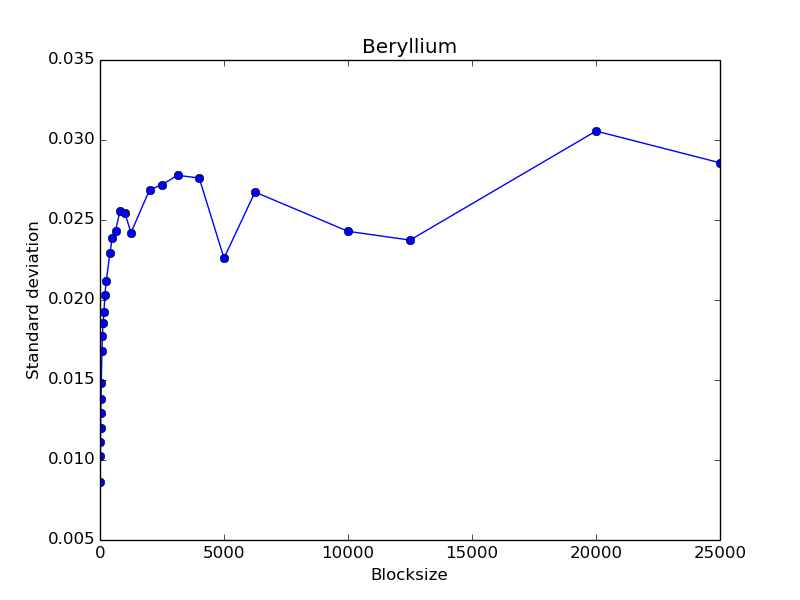
\includegraphics[width=0.45\linewidth]{../figures/Beryllium_blocking}
			\centering 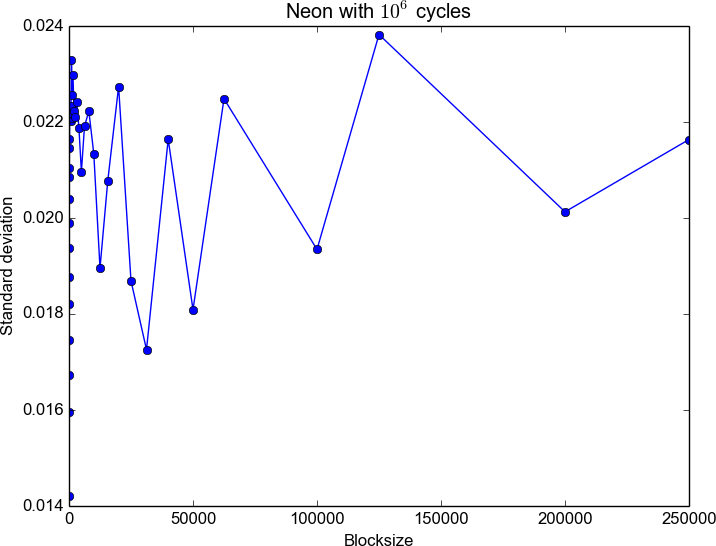
\includegraphics[width=0.45\linewidth]{../figures/Neon_blocking}
			\protect\caption{STD vs. blocksize with $10^{6}$ MC cycles.  The STD should have a plateauing trend as the blocksize increases.} \label{fig01:std_Stuff}
		\end{figure}

	\subsection{Verification of the model}
		\subsubsection{Verification of the general Monte Carlo method}
			The wavefunction for a Hydrogen atom is known, see equation \eqref{eq:hydrogen}, a Monte Carlo calculation for an exact wavefunction will give a exact result.

			\begin{align}
				 \Psi(\rho ) = \alpha \rho e^{-\alpha\rho} \qquad \text{ With  local energy: } \qquad E_{L} (\rho) = - \frac{1}{\rho} - \frac{\alpha}{2} \left( \alpha - \frac{2}{\rho} \right) \label{eq:hydrogen}
			\end{align}

			If the VMC calculation is run with a Hydrogen atom with \(\alpha = 1\) it should produce an energy of exactly \( -0.5\) with \(0\) variance. A check for this is implemented as a unit test in the program.

			The closed expressions of the local energy has also been verified by comparing them to numerical versions and checked that they produced similar values.

		%Need to check up some stuff when including this.
		\subsubsection{Verification of the Slater determinant and the laplacian Slater determinan ratio}
			To verify that the Slater determinant part of the trialfunctions is working correctly we use the fact that the states for a hydrogen atom can be calculated analytically, see for example Griffiths textbook  \cite{griffiths2005introduction}, and is given by
			\begin{align}
				E_n = -\frac{E_1}{n^2}  \qquad \text{; where } n  \text{ is the main state number}
			\end{align}

			By considering the other atoms without interaction between the electrons we can achieve an analytical solution by the same method.
			\begin{center}
				\begin{tabular}{| c | c |}
				\bottomrule
				Atom & Energy
				\\ \hline
				Hydrogen 	& \( E_1 = -\frac{1}{2} \)
				\\ \hline
				Helium 		& \( E_1 = -4\)
				\\ \hline Beryllium		& \( E_1 = -20 \)
				\\ \hline Neon		& \( E_1 = -200 \)
				\\ \toprule
				\end{tabular}
			\end{center}

		\subsubsection{Verification of the Padè-Jastrow part.}
			To verify that the part of the code that treats the correlation part of the kinetic energy we calculate, we check that it reproduces the correct results in the total energy and variation, but we also perform some tests on various parts by considering the Helium atom, where we calculate certain parts of the sums by hand and then compare the results with the ones given by the ratio machinery.

			Let us consider the gradient ratio of the Padè-Jastrow factor in Helium, \(\frac{\nabla\psi_C(\vb{r}_{12})}{\psi_C(\vb{r}_{12})}\) with \(\psi_C(\vb{r_{12}}) = e^{\frac{r_{12}}{2(1+\beta r_{12})}}\). Using the results from equation \eqref{eq:gradient_ratio_Jastrow} on Helium we get

			\begin{align}
				\frac{\nabla\Psi_C}{\Psi_C} &= \frac{1}{\Psi_c} \pdv{\Psi_C}{x_k} = \frac{\vb{r_{12}}}{r_{12}}\pdv{}{r_{12}}\left( \frac{r_{12}}{2(1+\beta r_{12})} \right) - \frac{\vb{r_{21}}}{r_{21}}\pdv{}{r_{21}}\left( \frac{r_{21}}{2(1+\beta r_{21})} \right)
				\\
				&= 2\frac{\vb{r_{12}}}{r_{12}}\pdv{}{r_{12}}\left( \frac{r_{12}}{2(1+\beta r_{12})} \right)
				\\
				&= \frac{\vb{r_{12}}}{r_{12}} \frac{1}{(1+\beta r_{12})^2}
			\end{align}

			Testing that the program reproduces this for the helium atom indicates the \(\frac{\nabla \Psi_C}{\Psi_C}\) is being calculated correctly.

\section{Results}
	\subsection{Variational Monte Carlo calculations of the helium
atom}
		As a first attempt to solve the ground state energy for the helium
		atom we perform Variational Monte Carlo calculation with a brute force
		Metropolis sampling. We do this with two trial wave functions
		\[
		\psi_{T1}({\bf r_{1}},{\bf r_{2}},{\bf r_{12}})=\exp{\left(-\alpha(r_{1}+r_{2})\right)}
		\]
		and
		\[
		\psi_{T2}({\bf r_{1}},{\bf r_{2}},{\bf r_{12}})=\exp{\left(-\alpha(r_{1}+r_{2})\right)}\exp{\left(\frac{r_{12}}{2(1+\beta r_{12})}\right)},
		\]
		using $\alpha$ and $\beta$ as variational parameters. Energy values
		for the simple wave function, $\psi_{T1}$, using only one variational
		parameter $\alpha$, are shown in figure \ref{fig01:alpha_Simple}.
		We run the Variational Monte Carlo calculation with $10^{7}$ cycles.
		As we see in the figures, the energy minimum occurs when we use $\alpha=1.65$.
		Using this value for $\alpha$ we get an energy of $-2.8442934$.
		The parameter $\alpha$ can be interpreted as a parameter for the
		force pulling the electron to the nucleus.

\subsection{First part}

	As a first attempt to solve the ground state energy for the helium
	atom we perform Variational Monte Carlo calculation with a brute force
	Metropolis sampling. We do this with two trial wave functions
	\[
	\psi_{T1}({\bf r_{1}},{\bf r_{2}},{\bf r_{12}})=\exp{\left(-\alpha(r_{1}+r_{2})\right)}
	\]
	and
	\[
	\psi_{T2}({\bf r_{1}},{\bf r_{2}},{\bf r_{12}})=\exp{\left(-\alpha(r_{1}+r_{2})\right)}\exp{\left(\frac{r_{12}}{2(1+\beta r_{12})}\right)},
	\]
	using $\alpha$ and $\beta$ as variational parameters. Energy values
	for the simple wave function, $\psi_{T1}$, using only one variational
	parameter $\alpha$, are shown in figure \ref{fig01:alpha_Simple}.
	We run the Variational Monte Carlo calculation with $10^{7}$ cycles.
	As we see in the figures, the energy minimum occurs when we use $\alpha=1.65$.
	Using this value for $\alpha$ we get an energy of $-2.8442934$.
	The parameter $\alpha$ can be interpreted as a parameter for the
	force pulling the electron to the nucleus.

	\begin{figure}
	\centering 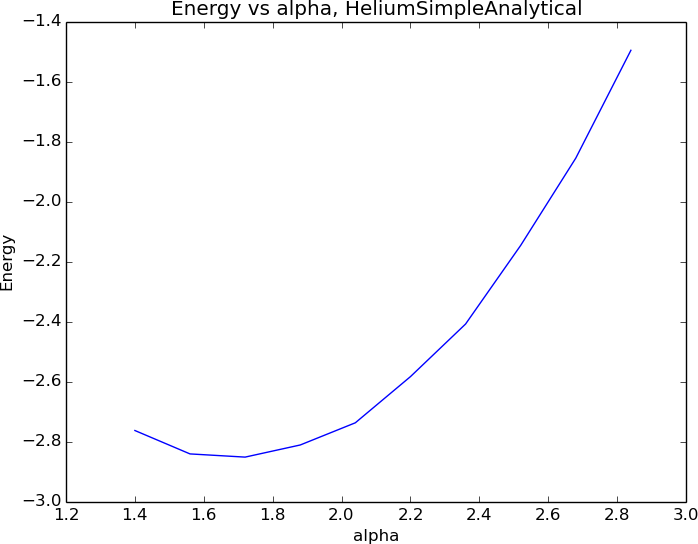
\includegraphics[width=0.45\linewidth]{../figures/EnergyVsAlphaHeliumSimpleAnalytical}
	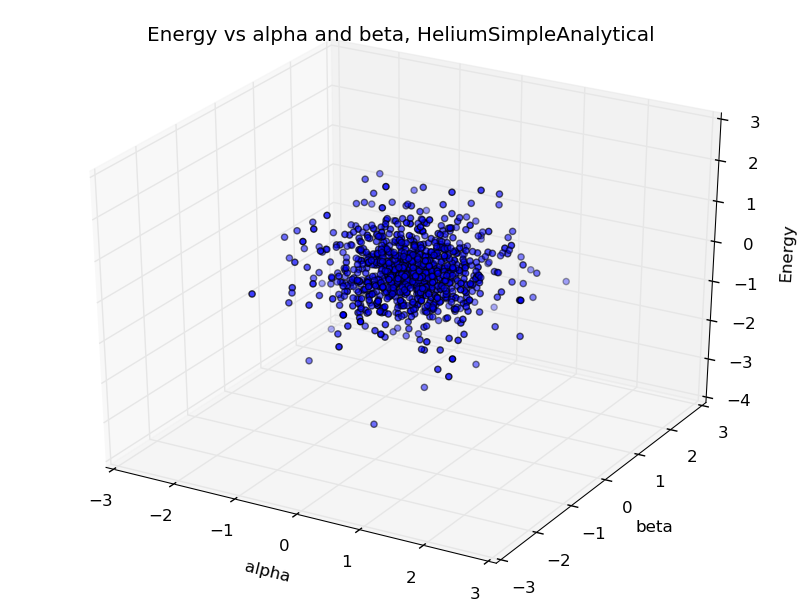
\includegraphics[width=0.45\linewidth]{../figures/VarianceVsAlphaHeliumSimpleAnalytical}

	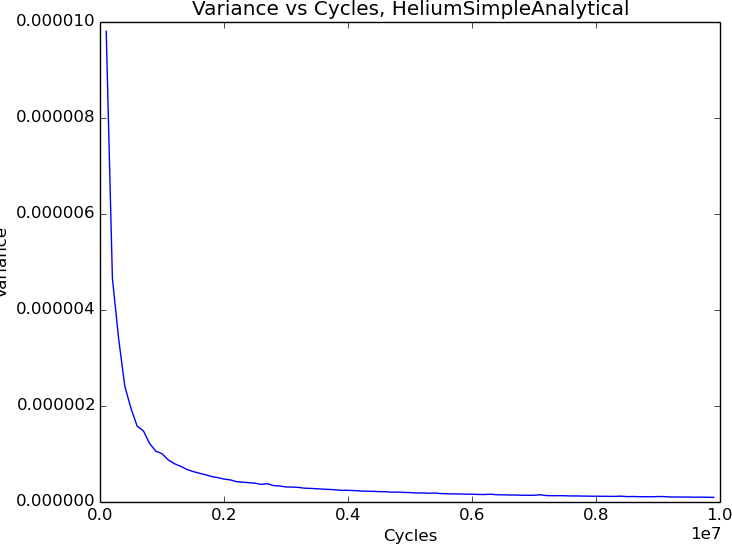
\includegraphics[width=0.45\linewidth]{../figures/VarianceNCyclesHeliumSimpleAnalytical}\protect\protect\caption{Plots for Helium $\psi_{T1}$ for energy versus $\alpha$, variance versus $\alpha$, and variance as function of Monte Carlo cycles.}
	\label{fig01:alpha_Simple}
	\end{figure}


	\begin{figure}
	\centering 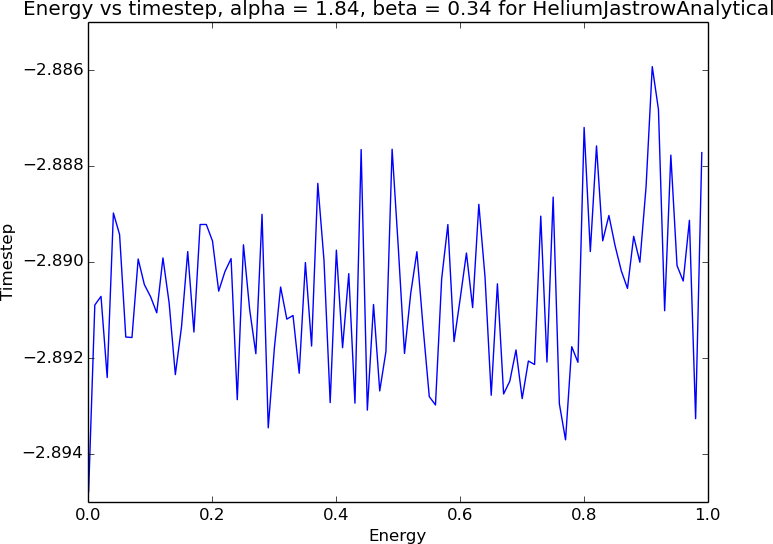
\includegraphics[width=0.45\linewidth]{../figures/HeliumJastrowAnalyticalTimeEnergy}
	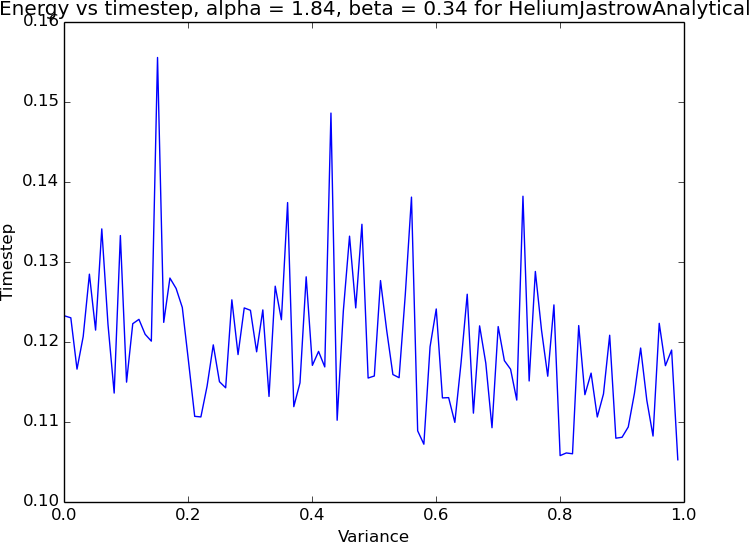
\includegraphics[width=0.45\linewidth]{../figures/HeliumJastrowAnalyticalTimeVariance}
	\protect\caption{Plots for Helium $\psi_{T2}$ for the energy versus the timestep, and the variance versus the timestep.}
	\label{fig02:timestep}
	\end{figure}

	We now look at our second trial function, $\psi_{T2}$. Running over
	different values for the two variables $\alpha$ and $\beta$, again
	with $10^{7}$ cycles in the Monte Carlo simulation, we get the results
	presented in figure \ref{fig03:AlphaBeta}. From this run we find
	that the optimal values are $\alpha=1.8$ and $\beta=0.94$, and we
	get a minimum energy of $-2.8979105$, which is considerably better
	than without the Jastrow factor.

	\begin{figure}
	\centering 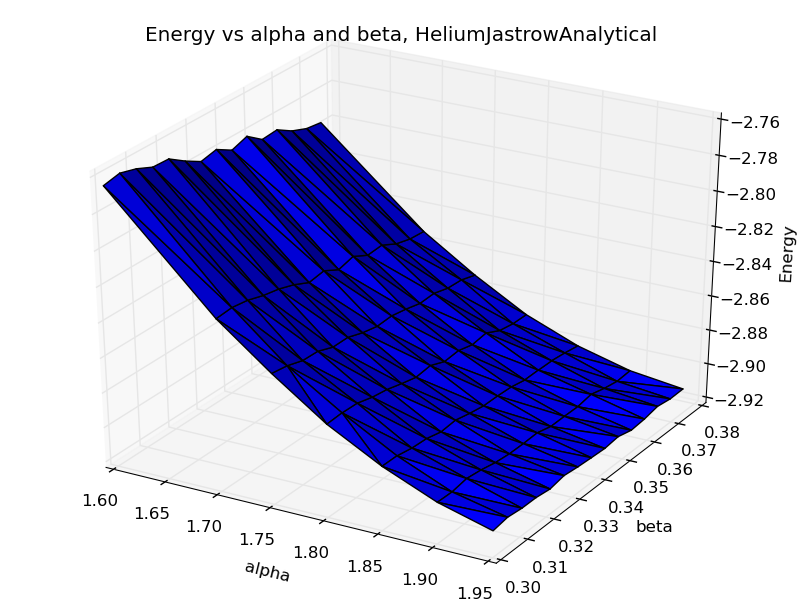
\includegraphics[width=0.45\linewidth]{../figures/HeliumJastrowAnalyticalAlphaBetaEnergy}
	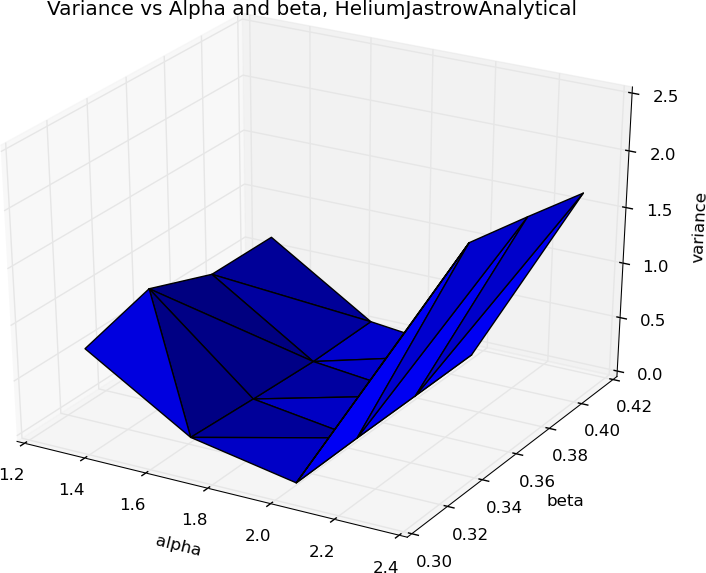
\includegraphics[width=0.45\linewidth]{../figures/HeliumJastrowAnalyticalAlphaBetaVariance}
	\protect\caption{Using $\psi_{T2}$, plot of the energy versus alpha and beta, and plot of the variance versus $\alpha$ and $\beta$. }
	\label{fig03:AlphaBeta}
	\end{figure}

	Finally we use our Variational Monte Carlo machinery to find the ground
	state energy for a beryllium atom. Since beryllium has 4 electrons,
	compared to the 2 in helium, the computation is much slower and we
	only had time to run it for $10^{6}$ cycles. We then find the lowest
	energy to be $-14.4127$ with $\alpha=3.8$ and $\beta=0.293$.

	From reseach papers we find the value for energy in the ground state
	of helium to be $-2.9037$ \cite{Kinoshita:1957:PR} and the value
	for energy in the ground state of beryllium to be $-14.667$ \cite{Koput:2011:PCCP}.
	Koput{]}. In table (\ref{tab:energyReference1}) we compare results
	obtained with our Variational Monte Carlo method with results from
	various research papers.

	\begin{table}
		\centering
		\begin{tabular}{|c|c|c|}
			\hline
			Atom & VMC & References\tabularnewline
			\hline
			\hline
			Helium $\psi_{T1}$ & $-2.8442$ & $-2.9037$ \tabularnewline
			\hline
			Helium $\psi_{T2}$ & $-2.8979$ & $-2.9037$ \tabularnewline
			\hline
			Beryllium & $-14.4127$ & $-14.667$\tabularnewline
			\hline
		\end{tabular}

		\protect
		\caption{Comparison of energies found with Variational Monte Carlo method and
		energies found in research papers.}
		\label{tab:energyReference1}
	\end{table}

	\subsubsection{Alpha and Beta Values}

		\begin{table}
			\center
			\begin{tabular}{| c | c| c |}
			    \hline
			   	\textbf{Trialfunction} & \(\mathbf{\alpha}\) & \(\mathbf{\beta}\)
			    \\ \hline
			    Helium $\psi_{T1}$ & 1.65 & -
			    \\ \hline
			    Helium $\psi_{T2}$ & 1.8 & 0.94
			    \\	\hline
			    Beryllium $\psi_{T2}$	& 3.8	&	 0.293
			    \\ \hline
	  		\end{tabular}
	  		\caption{The values for \(\alpha\) and \( \beta \) where found by doing running Monte Carlo calculation with over a mesh of different \(\alpha\) and \( \beta \) values, with stepssize \(0.02\). Each Monte Carlo run went over \(10 000 	000\), using importance sampling. Then the run with the lowest energy gave the \(\alpha\) and \(\beta\) values.}
		  	\label{tab:alpha_beta1}
		\end{table}

		Table \ref{tab:alpha_beta1} shows the values, for \(\alpha\) and \(\beta\) values, we got from  running several Monte Carlo cycles with different values. As an algorithm to pick out the best values we minimized the energy found in the Monte Carlo runs. The values found are quite uncertain since the variance of the energy was quite high compared to the difference caused by varying the parameters. The variance was more smooth as a function of the parameters, see fig \ref{fig03:AlphaBeta} and should have been used.




			\subsubsection{Computational speed gain by using an analytical local energy}
				By using an analytical expression for the local energy instead of using a numerical derivation in the calculation a speed up of approximately factor \(4\) was achieved, see table \ref{tab:analyticVSNumeric}.


				\begin{table}
					\center
					\begin{tabular}{| c | c | c | c |}
					    \hline
					   	\textbf{Trialfunction} & Numerical (s) & Analytical (s) & Ratio
					    \\ \hline
					    Helium $\psi_{T1}$ & 61.75 & 14.34 & 4.307
					    \\ \hline
					    Helium $\psi_{T2}$ & 86.76 & 19.98	& 4.342
					    \\	\hline
					    Beryllium $\psi_{T2}$ & 1918.34  &	 &
	 				    \\ \hline
					\end{tabular}
					\caption{The time to run a Monte Carlo run with \(10^7\) cycles. The closed expression for the local energy increased the computation time by a significant degree for each trialfunction. }
					\label{tab:analyticVSNumeric}
				\end{table}

	\subsection{Variational Monte Carlo calculations of the Beryllium and Neon atoms}

		\begin{table}
			\center
				\begin{tabular}{|c|c|c|}
				    \hline
				   	Atom & VMC & References
				    \\ \hline
				    Beryllium & $-14.3888$ & $-14.667$
				    \\ \hline
				    Neon & $-127.961$ &  \(-128.928\)
				    \\	\hline
			  \end{tabular}
			  \caption{Comparison of energies found with Variational Monte Carlo method and
			energies found in research papers \cite{Koput:2011:PCCP} \cite{QUA:QUA560090204} }
			\label{tab:energyReference}
		\end{table}

		We attempt to solve the ground state energy for the Beryllium atom and Neon atom using a Variational Monte Carlo calculation with importance sampling. We have used the trial functions \eqref{eq:BerylliumTrialFunction} for Beryllium and \eqref{eq:NeonTrialFunction} for Neon which uses $\alpha$ and $\beta$ as variational parameters.

		For Beryllium we have the Alpha and Beta values $\alpha=4.0$ and $\beta=0.31$. We use $10^{6}$ cycles and find the energy to be $-14.3795$, with a variance of $0.0020$.
		For Neon, with $5 \times 10^{5}$ cycles we get an energy of $-127.936$ with a variance of $0.0548$.

		From reseach papers we find the value for energy in the ground state
		of Beryllium to be $-14.667$ \cite{Koput:2011:PCCP} and the value
		for energy in the ground state of Neon to be \(-128.928\) \cite{QUA:QUA560090204}.
		In table \ref{tab:energyReference} we compare results
		obtained with our Variational Monte Carlo method with results from
		various research papers.


		\subsubsection{Alpha and Beta Values}
			\begin{table}
			\center
					\begin{tabular}{| c | c| c |}
					    \hline
					   	\textbf{Trialfunction} & \(\mathbf{\alpha}\) & \(\mathbf{\beta}\)
					    \\ \hline
					    Beryllium $\psi_{T2}$	& 3.8	&	 0.293
					    \\ \hline
					    Neon $\psi_{T2}$	&	10.22	&	0.091
					    \\	\hline
				  \end{tabular}
				  \caption{The values for \(\alpha\) and \( \beta \) where found by doing running Monte Carlo calculation with over a mesh of different \(\alpha\) and \( \beta \) values. For Beryllium each Monte Carlo run went over \(10 000 000\), using importance sampling. For Neon each run went over \(5 000\), also with importance sampling. Then the run with the lowest energy gave the \(\alpha\) and \(\beta\) values.}
				  \label{tab:alpha_beta}
			\end{table}

			\begin{figure}
				\centering 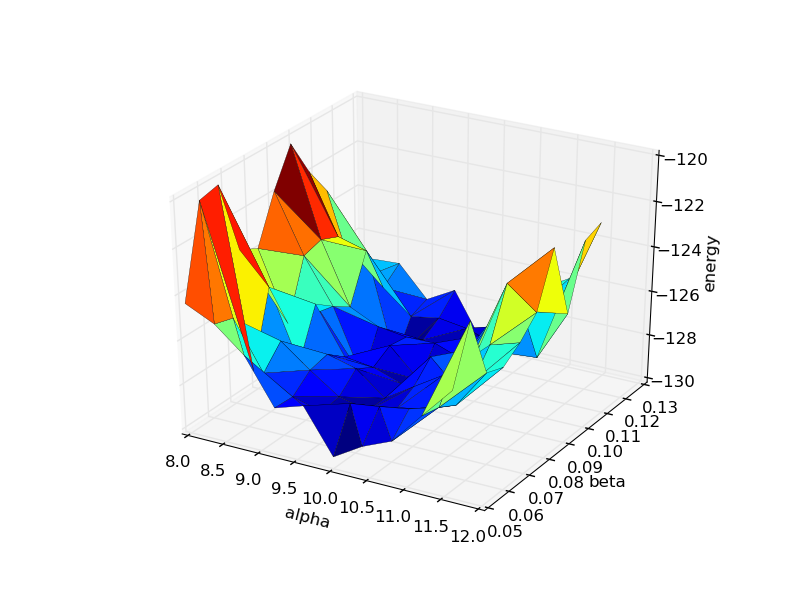
\includegraphics[width=0.45\linewidth]{../figures/Neon_alpha_beta}
				\centering 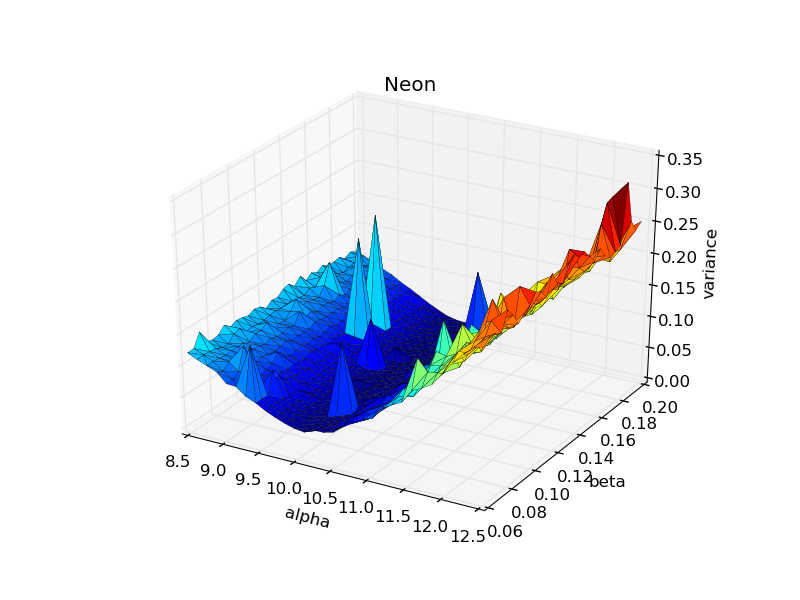
\includegraphics[width=0.45\linewidth]{../figures/Neon_alpha_beta_var}
				\protect\caption{Energy (left) and variance (right) for different Alpha and Beta values for Neon.}
				\label{fig:alpha_beta_comparison}
			\end{figure}

			We use Alpha and Beta values for Beryllium found in project 1, so the only Alpha and Beta values we have to find are for Neon. Table \ref{tab:alpha_beta} shows the values, for \(\alpha\) and \(\beta\) values, we got from  running several Monte Carlo cycles with different values. As an algorithm to pick out the best values we minimized the energy found in the Monte Carlo runs. The values found are quite uncertain since the variance of the energy was quite high compared to the difference caused by varying the parameters. A plot of different energies and variance given by different Alpha and Beta values are shown in figure \ref{fig:alpha_beta_comparison}.

		\subsubsection{Speedup with MPI}
			\begin{table}
			\center
					\begin{tabular}{| c | c| c| c| c|}
					    \hline
					   	\textbf{Num. of processes} &	1	&	2	&	3	&	4
					    \\ \hline
					    \textbf{Speedup}	&	1.0	&	1.97	&	2.90	&	3.35
					    \\	\hline
				  \end{tabular}
				  \caption{MPI speedup}
				  \label{tab:MPI_speedup}
			\end{table}

			\begin{figure}
			\centering 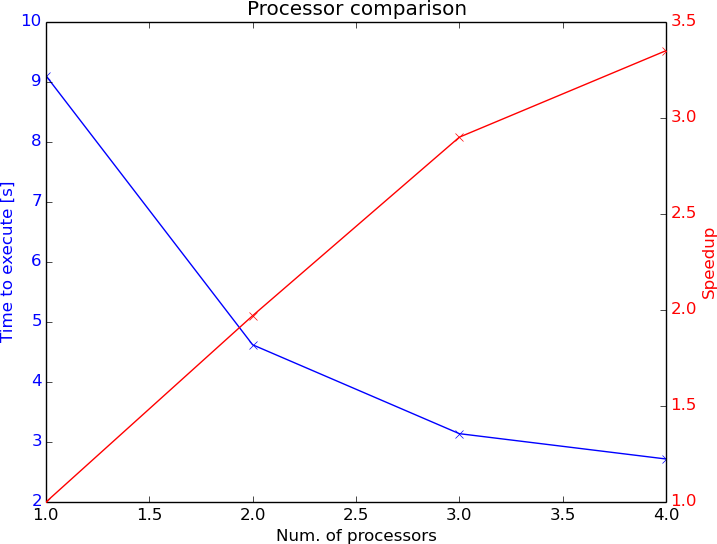
\includegraphics[width=0.45\linewidth]{../figures/processor_number_time_comparison}
			\protect\caption{MPI speedup}
			\label{fig:MPI_speedup}
			\end{figure}

			It is desirable to have a speedup as close as possible to the number of processors used. The speedup measured by our VMC program running 1, 2, 3 and 4 is shown in table \ref{tab:MPI_speedup} and figure \ref{fig:MPI_speedup}. We see that the speedup is good for 2 and 3 processes, but for 4 processes suffers somewhat because it also have to run the OS and other programs.

		\subsubsection{Onebody densities / Comparisons / Without Jastrow}
			As we see in the verification section, without interaction the energies behave like hydrogen like wave functions. Comparing with the energies we obtain when also using interaction in the calculations we see that the Jastrow factor offers a good improvement on the energy, especially for larger systems.

		\subsubsection{Charge Density}
			The charge density gives measure of how often the electrons occupies certain area in the Monte Carlo simulation, in figure \ref{fig:charge_density} the square of the norm of the distance is plotted.
			On the Neon atom the electrons have a closer distribution to the center that is caused by the more electrically charged core of Neon compared to Beryllium.

			\begin{figure}
				\centering 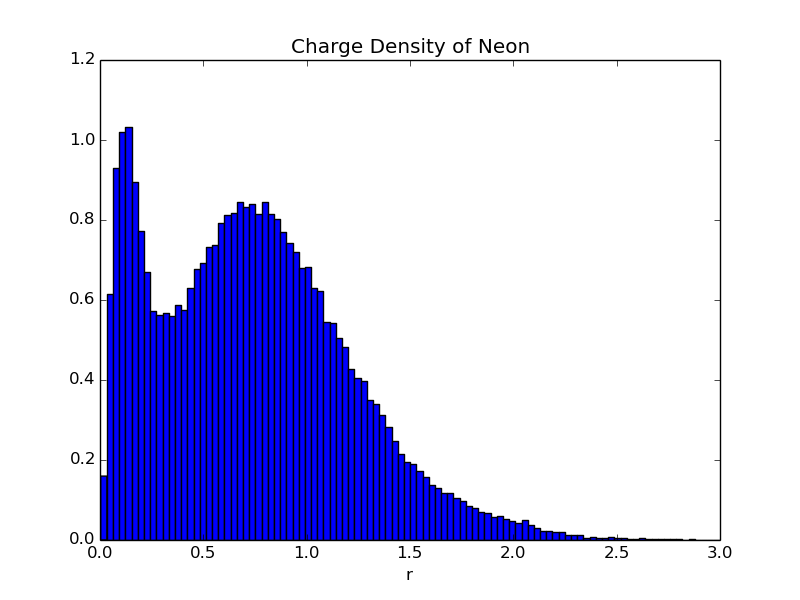
\includegraphics[width=0.45\linewidth]{../figures/ChargeDensityNeon}
				\centering 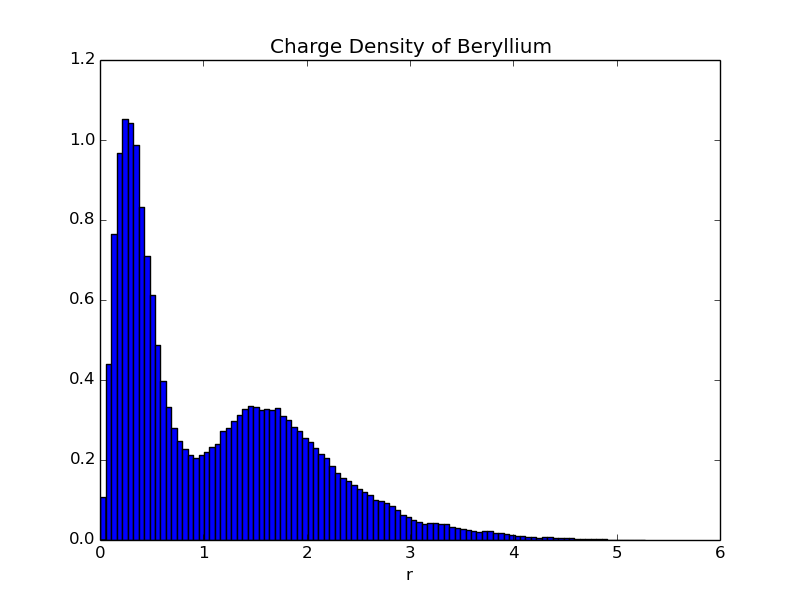
\includegraphics[width=0.45\linewidth]{../figures/ChargeDensityBeryllium}
				\protect\caption{Charge densities for Neon and Beryllium with the x-axis representing how far away from the atomcenter the electrons are. }
				\label{fig:charge_density}
			\end{figure}

\section{Conclusions and discussion}
	\subsection{Critique on the exercise}


\appendix

\section{Program overview}

	\begin{figure}
		\begin{tikzpicture}[%
		    >=triangle 60,              % Nice arrows; your taste may be different
		    start chain=going below,    % General flow is top-to-bottom
		    node distance=6mm and 45mm, % Global setup of box spacing
		    every join/.style={norm},   % Default linetype for connecting boxes
		    ]
		% ------------------------------------------------- 
		% A few box styles 
		% <on chain> *and* <on grid> reduce the need for manual relative
		% positioning of nodes
		\tikzset{
		  base/.style={draw, on chain, on grid, align=center, minimum height=4ex},
		  proc/.style={base, rectangle, text width=10em},
		  test/.style={base, diamond, aspect=2, text width=5em},
		  term/.style={proc, rounded corners},
		  % coord node style is used for placing corners of connecting lines
		  coord/.style={coordinate, on chain, on grid, node distance=6mm and 45mm},
		  % nmark node style is used for coordinate debugging marks
		  nmark/.style={draw, cyan, circle, font={\sffamily\bfseries}},
		  % -------------------------------------------------
		  % Connector line styles for different parts of the diagram
		  norm/.style={->, draw, lcnorm},
		  free/.style={->, draw, lcfree},
		  cong/.style={->, draw, lccong},
		  it/.style={font={\small\itshape}}
		}
		% -------------------------------------------------
		% Start by placing the nodes
		\node[proc, densely dotted, it] (init) {Initialize solver};
		\node[term, join] (split)      {Split into several threads for multi core};
		\node[term, join] (position)      {Suggest move};
		\node[term, join] (SD) { Compute/update \( |D| \) };
		\node[term, join ] (metro) {Compute Metropolis Ratio};
		\node[test, densely dotted , join ]	(test)	{\(R \ge r\)};
		\node[term]	(new_pos)	{\(\vb{r}^{old} = \vb{r}^{new}\)};
		\node[term, join ]	(energy)	{ Store \(E_L\) };
		\node[test, densely dotted ,join ]	(last)	{Last cycle?};
		\node[term]	(end)	{Collect samples};


		%Setting up the nodes on the side
		\node [term, right=of SD] (trialfunction) {Compute \( \psi_T(\vb{r}) \)};
		\node [term, left=of SD] (quantum) { Compute  Quantumforce};
		\node[term, left=of test] (old_pos) {Keep \(  \vb{r}^{old} \)};
		\node [coord, left=of new_pos] (c1)  {};    
		\node[coord, right=of last]	(around1){};
		\node[coord, right=of around1] (around2) {};
		\node[coord, right=of position]	(around3){};
		\node[coord, right=of around3]	(around4){};


		%Draw new links between boxes
		% \path (SD.south) to node [near start, xshift=1em] {$y$} (quantum);
		\draw [->,lcnorm] (SD.west) -- (quantum);
		\draw [->,lcnorm] (SD.east) -- (trialfunction);
		\draw [->, lcnorm] (quantum.south) -- (metro);
		\draw [->, lcnorm] (trialfunction.south) -- (metro);
		\draw [*->, lccong, , dotted] (test.west) -- (old_pos);
			\path (test.west) to node [ yshift = -1em] {no} (old_pos);
		\draw [*->, lcfree, dotted] (test.south) -- (new_pos);
			\path (test.south) to node [xshift = -1em]{yes} (new_pos);

		\draw [-, lcnorm] (old_pos.south) -- (c1);
		\draw [->, lcnorm] (c1.south) -- (energy);

		\draw[*-, lccong, dotted] (last.east) -- (around2);
			\path (last.east) to node [yshift = -1em] {no} (last);
			\draw[-, lccong, dotted] (around2.east) -- (around4);
			\draw[->, lccong, dotted] (around4) -- (position);

		\draw [*->, lcfree, dotted] (last.south) -- (end);
			\path (last.south) to node [xshift = -1em]{yes} (new_pos);


		\end{tikzpicture}
		\caption{Schematic overview over the workflow of the VMC solver}
		\label{fig:schematic}
	\end{figure}

	\begin{figure}
		\begin{tikzpicture}[%
			    >=triangle 60,              % Nice arrows; your taste may be different
			    start chain=going below,    % General flow is top-to-bottom
			    node distance=6mm and 45mm, % Global setup of box spacing
			    every join/.style={norm},   % Default linetype for connecting boxes
			    ]
			% ------------------------------------------------- 
			% A few box styles 
			% <on chain> *and* <on grid> reduce the need for manual relative
			% positioning of nodes
			\tikzset{
			  base/.style={draw, on chain, on grid, align=center, minimum height=4ex},
			  proc/.style={base, rectangle, text width=10em},
			  test/.style={base, diamond, aspect=2, text width=5em},
			  term/.style={proc, rounded corners},
			  % coord node style is used for placing corners of connecting lines
			  coord/.style={coordinate, on chain, on grid, node distance=6mm and 45mm},
			  % nmark node style is used for coordinate debugging marks
			  nmark/.style={draw, cyan, circle, font={\sffamily\bfseries}},
			  % -------------------------------------------------
			  % Connector line styles for different parts of the diagram
			  norm/.style={->, draw, lcnorm},
			  free/.style={->, draw, lcfree},
			  cong/.style={->, draw, lccong},
			  it/.style={font={\small\itshape}}
			}

			%Center column
			\node[term, fill=lcfree!25,  align=center] (solver) {VMCSolver};
			\node[coord]	(blank)	{};
			\node[term] (trialfunction)	{Trialfunction};
				\draw[->, lcnorm]	(solver.south) -- (trialfunction);
			\node[term, join]	(diff)	{He, Be, Ne, H\(_2\) or Be\(_2\)};


			%Sides with lines drawn
			\node[term, right=of blank] (derivatives) {Derivatives};
				\draw[->, lcnorm] (solver.east) -- (derivatives.west);

			\node[term, left=of blank] 	(slater)	{SlaterDeterminant};
				\draw[->, lcnorm] (solver.west) -- (slater.east);

			%Dotted lines between the connected classes
			\draw[-, lcfree, densely dotted] (slater.east) -- (derivatives.west);
			\draw[-, lcfree, densely dotted] (slater.east) -- (trialfunction.west);
			\draw[-, lcfree, densely dotted] (trialfunction.east) -- (derivatives.west);

		\end{tikzpicture}

		\caption{Class and subclass structure used by the program}
		\label{fig:classes}
	\end{figure}





\bibliography{bibliography}
\bibliographystyle{plain}


\end{document}